

\documentclass[twocolumn,12pt,journal,final]{IEEEtran_modified}
\usepackage{graphicx}
\usepackage{caption}
\usepackage{float}
\linespread{1.3}
 \setlength{\parskip}{0ex plus 0.0ex minus 0.0ex}

\begin{document}

\title{CS3243: Introduction to AI\\ Let’s Play Tetris! }

\author{
  Group 13 \\
  Bjoern Jesper Andersson (A0118441), Le Viet Bach (A0088827L) \\ Daniel Gunnarsson (A0118309H), Zeng Qingtao (A0098924M) \\
  2014-04-18 \\ 
}

\maketitle

\section{Introduction} 
The purpose of the project is to create a utility-based agent whose goal is to obtain a maximal amount of rows cleared in the game of Tetris. The agent created uses a heuristic function that has been improved through the use of a genetic algorithm. The average amount of rows cleared in a normal game of Tetris for the resulting agent is approximately 230,000.

\section{Strategy} 
For every turn, all possible moves (orientations and positions) of the new block is evaluated using an utility function. The move with the highest utility will be chosen.

The utility function is a weighted sum of different features of the board after a move is played. Generally, “positive features” such as number of rows cleared that turn are given positive weights and “negative features” such as column heights are given negative weights. The actual weight for each function is determined using a genetic algorithm.

The following sections will provide more details of our implementation.

\subsection{Features}
The following are the characteristics that are evaluated in the heuristic function. They are given by their name in the program followed by an explanation of their purpose. More features were tested but discarded when they did not show to provide a better result for the current set of features.

\begin{itemize}
  \item \textbf{Roughness} - Sum of height difference between all pairs of adjacent columns.
  \item \textbf{MaxColumnHeight} - The maximum column height of the state.
  \item \textbf{NumRowsCleared} - Number of rows cleared.
  \item \textbf{HasLost} - Whether the move results in a loss or not.
  \item \textbf{NumFaults} - Number of holes, a hole is an empty block with a non-empty block above it.
  \item \textbf{PitDepths} - Depth of pits, a pit is a column with adjacent columns higher by at least two blocks and the pit depth is defined as the difference between the height of the pit column and the shortest adjacent column.
  \item \textbf{MeanHeightDifference} - Mean height difference, the average of the difference between the height of each column and the mean height of the state. 
\end{itemize}

\subsection{Genetic Algorithm}
We used our own implementation of genetic algorithm where a chromosome is defined as a sequence of floats. A chromosome consists of 7 genes each corresponds to the weight of a feature.

For each generation, a set of 5 games, each consisting of 10,000,000 pieces generated. All chromosomes (or weight sets) are pitted against these sequences. The average number of rows a weight set can clear is its fitness score.

From the initial population of 100, chromosomes are selected using a roulette wheel to create a new generation. The genetic algorithm used one-point cross-over with a rate of 0.6 and a mutation rate of 0.01. To detect convergence, it keeps track of the highest fitness score in each generation. After 20 generations where there is no increase in maximum fitness, the algorithm terminates and reports the fittest chromosome.

\subsection{Parallel processing}

Since the AI agent and especially the genetic algorithm have a lot of data to process, we decided to use parallel processing to speed it up.

It is clear that two board states are independent and they can be evaluated in parallel with each other. The same is true for weight sets (chromosomes). This is, thus, an “embarrassingly parallel” problem.

Since the provided State class does not allow retracting a move, we created our own class $ImmutableState$ which takes in the current state as a parameter and copies it into an identical structure as the one provided for the project. It returns the result of a move and does not change its internal state. Being immutable, it can be safely used and shared in a multithreaded context without any locking.

A simple implementation of MapReduce, using $java.util.concurrent.ForkJoinPool$, was created so that we do not have to actually write any threaded code.

\section{Result}
The result presented in this section is from 100 runs of the weights shown in table 1. These were derived from a run of the genetic algorithm. The weights were obtained by taking the weights set provided in the constructor of the $PlayerSkeleton$ class multiplied by the modifiers in the functions for the features and then finally normalized. 

\begin{table}[h!]
\normalsize
  \begin{center}
    \begin{tabular}{| l | c |}
    \hline
    \textbf{Feature} & \textbf{Weight} \\
    \hline
    Roughness & 0.1242  \\ \hline
    MaxColumnHeight & 0.0307  \\ \hline
    NumRowsCleared & 0.0298  \\ \hline
    HasLost & 0.4959  \\ \hline
    NumFaults & 1 \\ \hline
    PitDepths & 0.3232  \\ \hline
    MeanHeightDifference & 0.3178  \\ \hline

    \end{tabular}
  \end{center}
  \caption{Weights for the features.}
  \label{tab:weights}
\end{table}

The distribution of results seen in figure 1 shows that most runs result in well below 200,000 rows cleared, but there are also three runs reaching above one million in rows cleared. The large difference between some of the neighbouring intervals are reasoned to be due to the relatively small data set.

\begin{figure}[H]
  \centering
    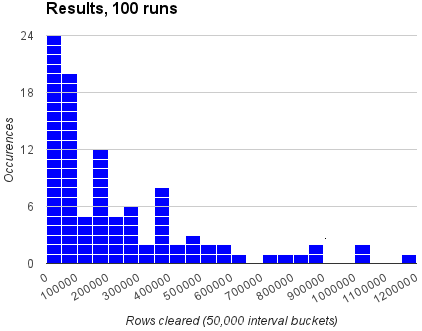
\includegraphics[width=0.5\textwidth]{bucketresults.png}
  \caption{Results from 100 runs, each block is one run.}
  \label{fig:bucketresults}
\end{figure}

The range of results is visualized in figure 2, with the median being slightly below 200,000 rows cleared. It also shows that the cluster of results decrease in size as the number of rows cleared increase. 

\begin{figure}[h]
  \centering
    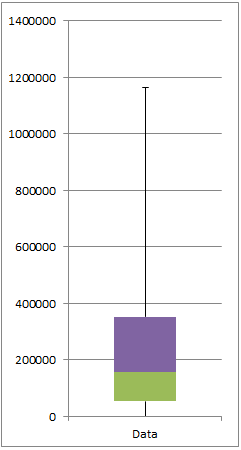
\includegraphics[scale=0.5]{blockresults.png}
  \caption{Block diagram showing the result.}
  \label{fig:blockresults}
\end{figure}

What is not obvious in figure 2 is that the lowest result obtained during the 100 runs was 116 rows cleared, as seen in table 2, while the best run reached 1,164,572 rows cleared. As already seen in figure 2, the average is well above the median value while the range of values is very large.

\begin{table}[h]
\normalsize
  \begin{center}
    \begin{tabular}{| l | c |}
    \hline
    \textbf{Metric} & \textbf{Value} \\
    \hline
    Average & 235323.2 \\ \hline
    Median & 156155.5 \\ \hline
    Max & 1164572 \\ \hline
    Min & 118 \\ \hline
    \end{tabular}
  \end{center}
  \caption{Common metrics for the 100 runs.}
  \label{tab:results}
\end{table}

\section{Discussion}

Many of the runs reach quite a low amount of rows cleared, these could possibly be due to some negative feature being missed in the implementation of the agent. Looking at these runs could yield some information about what combination of states and series of blocks that result in an early loss. Eliminating some of the worst cases would drastically increase the average score.

Another possible improvements could come from tweaking the genetic algorithm: by modifying the population as well as the cross-over and mutation rates.

Currently, the genetic algorithm can only run on one node. In the future, it could make use of MPI (message passing interface) to distribute the workload over a cluster and get the most out of a computing cluster such as Tembusu. It will greatly reduce computation time and allow more tweaking with the genetic algorithm’s parameters.

\end{document}


